\section{Corona Cruz Alan Gael}
\subsection{Definiciones}

\begin{enumerate}
    \item Exacto: Igual o que se asemeja en un grado muy alto a algo o alguien que es tomado como modelo. 
    \item Preciso: Dicho de una cosa: Perceptible de manera clara y nítida. 
    \item Estudio de movimientos y tiempos: Estudio de tiempos: actividad que implica la técnica de establecer un estándar de tiempo permisible para realizar una tarea determinada, con base en la medición del contenido del trabajo del método prescrito, con la debida consideración de la fatiga y las demoras personales y los retrasos inevitables.
Estudio de movimientos: análisis cuidadoso de los diversos movimientos que efectúa el cuerpo al ejecutar un trabajo. 
\end{enumerate}

\subsection{Objetivo}
\begin{enumerate}
    \item Durante el semestre se trabajara en un proyecto integrador el cual estara enfocado en realizar una practica de ensamble de un circuito, esto con el proposito de realizar un estudio de tiempos y movimientos, la practica sera de gran ayuda ya que podremos familiarizarnos con este tipo de procesos los cuales son habituales en la industria, para realizar esta practica tomaremos el papel de operario y observador, tambien se hara uso de herramientas de trabajo como lo son Overlief, Visual Studio Code y Solidworks, los cuales son herramientas que se usan dia a dia en un empleo para la realizacion de proyectos, el uso de estas sera de gran ayuda para tener un conocimiento de como trabajaremos en una empresa, asi como tener un conocimiento de sus ventajas y como se conectan entre si. 
 \end{enumerate}

\subsection{Material}

\begin{enumerate}
    \item Cables dupont: Es un cable con un conector en cada punta, que se usa normalmente para interconectar entre sí los componentes en una placa de pruebas. Se utilizan de forma general para transferir señales eléctricas de cualquier parte de la placa de prototipos.
    \ref{Cables}
\begin{figure}
    \centering
    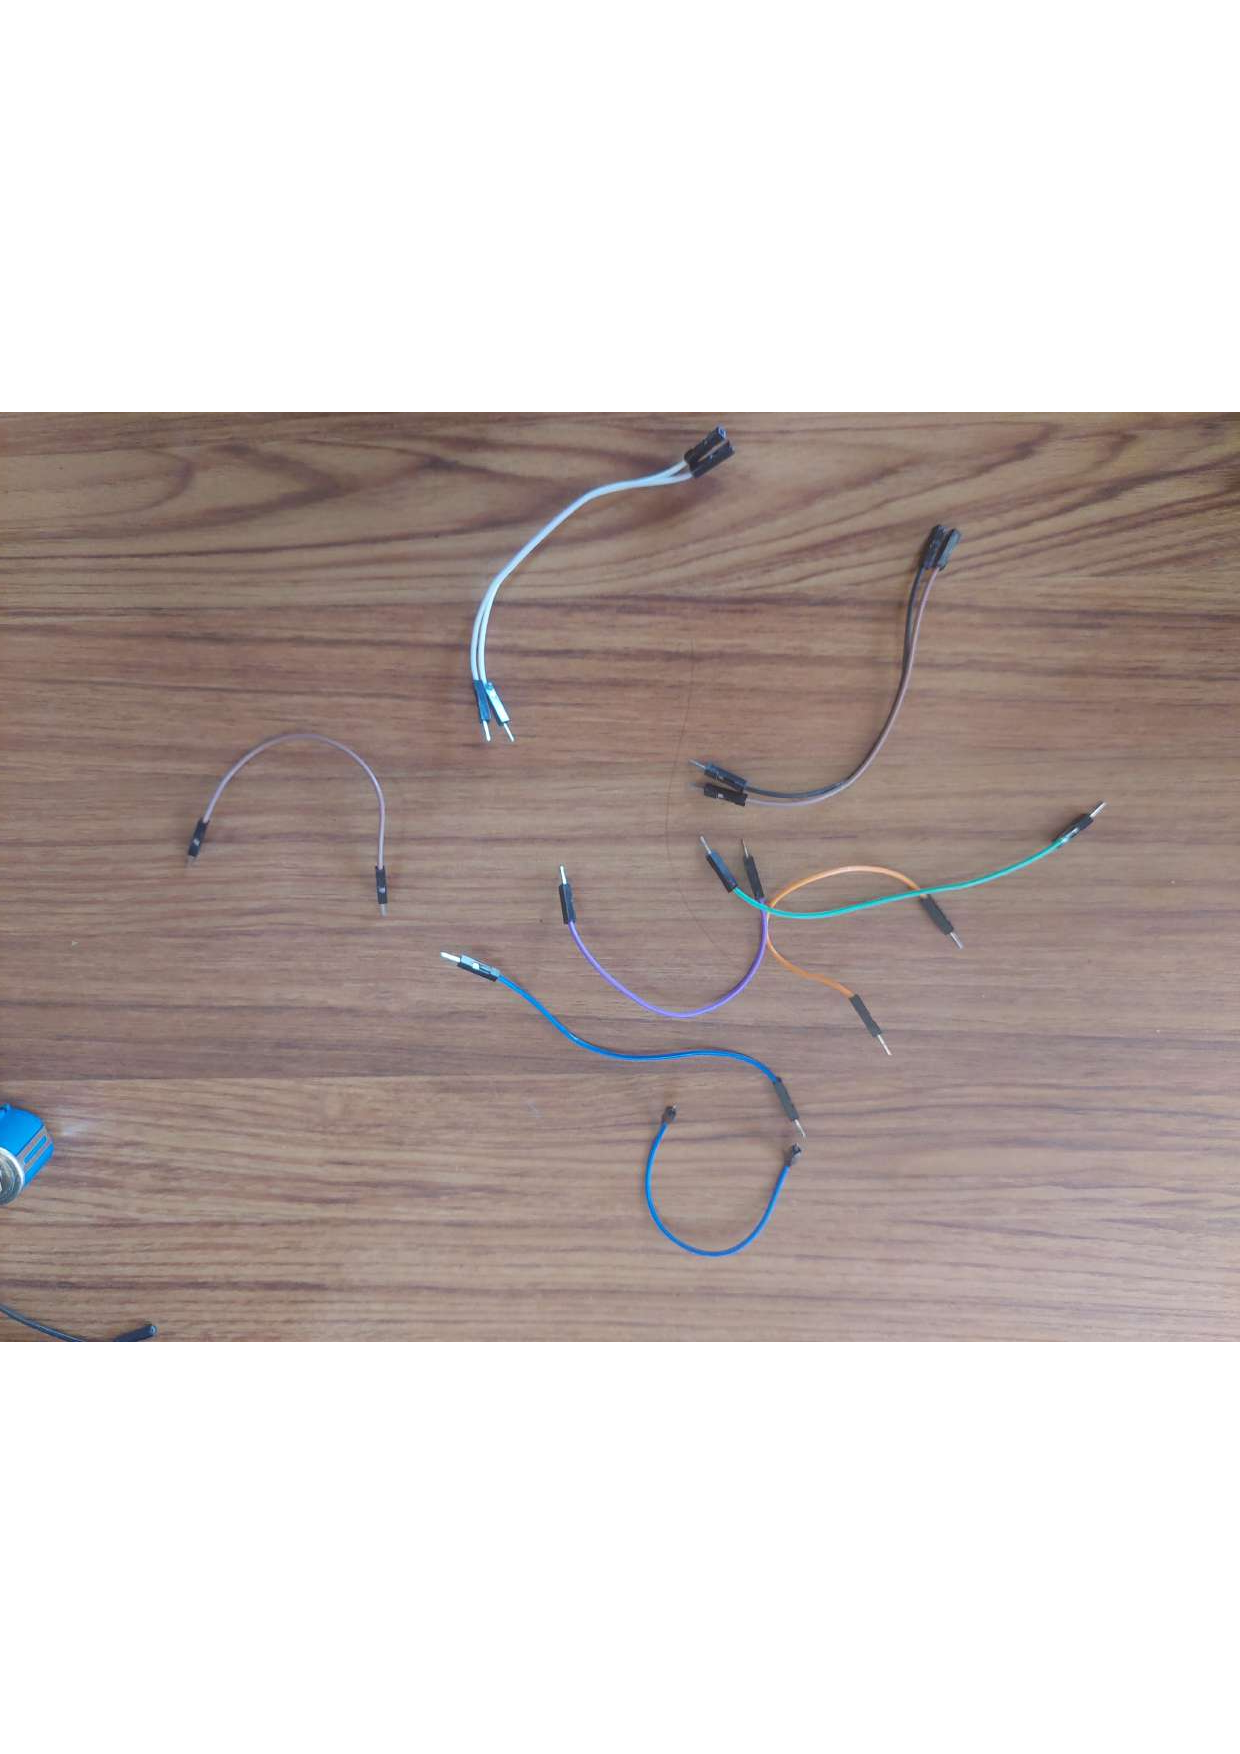
\includegraphics[scale=0.25]{8/Img/Img/Cables dupont.pdf}
    \caption{Cables dupont}
    \label{Cables}
\end{figure}
    \item Resistencias: Las resistencias son esenciales para facilitar el flujo adecuado de corriente. La resistencia sirve como un indicador que cuantifica qué tan rápido fluirá la corriente en un circuito utilizando ohmios como unidad.
    \item Protoboard: Es una herramienta simple que se usa en proyectos de robótica que permite conectar fácilmente componentes electrónicos entre sí, sin necesidad de realizar una soldadura.
    \item Arduino: Utilizado como un microcontrolador, cuando tiene un programa descargado desde un ordenador y funciona de forma independiente de éste, y controla y alimenta determinados dispositivos y toma decisiones de acuerdo al programa descargado e interactúa con el mundo físico gracias a sensores y actuadores.
    \item Potenciametro: Componente electrónico similar a los resistores pero cuyo valor de resistencia en vez de ser fijo es variable, permitiendo controlar la intensidad de corriente a lo largo de un circuito conectándolo en paralelo ó la caida de tensión al conectarlo en serie.
    \item Display: Dispositivo de ciertos aparatos electrónicos que permite mostrar información al usuario de manera visual o táctil.
\end{enumerate}

\subsection{Ensamble}
\begin{enumerate}
    \item Se instalara el arduino en el protoboard ensamblandolo en la linea con la letra b, insertandolo de izquiera a derecha 
    \item Tomaremos un cable dupont y lo colocaremos en el pin numero 7 del arduino, el otro extremo se colocara en la fila con la letra g dejando 2 espacios de donde termina el arduino
    \item Tomaremos otro cable dupont y lo colocaremos en el pin numero 6 del arduino, el otro extremo se colocara al lado derecho del cable dupont colocado anteriormente, dejando un espacio a su derecha
    \item Tomaremos otro cable dupont el cual se colocara en el pin con descripcion 3v3 del arduino, el otro extremo se instalara del lado positivo del protoboard en el segundo espacio de derecha a izquierda 
    \item Tomaremos otro cable dupont y lo colocaremos en el pin con descripcion G del arduino, el otro extremo se colocara en el primer espacio de izquierda a derecha del lado negativo 
\subsection{conexiones de display}   
    \item Tomaremos otro cable dupont el cual se colocara debajo del cable protoboard del segundo paso, el otro extremo se instalara en la parte trasera del display en el pin con descripcion SCL
    \item Tomaremos un nuevo cable dupont el cual se colocara debajo del cable dupont del tercer paso, el otro extremo se instalara en la parte trasera del display en el pin con descripcion SDA
    \item Tomaremos otro cable dupont el cual se colocara en el sexto espacio de derecha a izquiera del lado negativo del protoboard, el otro extremo se instalara en la parte trasera del display en el pin con descripcion GND
    \item Tomaremos otro cable dupont el cual se colocara arriba del cable dupont del paso anterior, el otro extremo se instalara en la parte trasera del display en el pin con descripcion VCC
\subsection{conexiones de potenciometro}
    \item Tomaremos un cable dupont el cual se colocara del lado positivo en el primer espacio de derecha a izquierda, el otro extremo se conectara con un nuevo cable dupont, el extremo sobrante se soldara al potenciometro 
    \item Tomaremos otro cable dupont el cual se colocara debajo del cable dupont del paso anterior, el cual terminara del lado negativo, el extremo de este se conectara de igual manera a un nuevo cable dupont y el extremo sobramte tambien se soldara al potenciometro
    \item Se conectara un ultimo cable dupont en el protoboard el cual ira en el pin 0 del arduino, posteriormente se soldara al potenciometro
\subsection{Resistencias}
    \item La primera resistencia se conectara debajo del cable dupont del paso numero 6 y el otro extremo se colocara en el lado positivo a 7 espacio a la izquierda del cable dupont del paso numero 9
    \item La segunda resistencia se colocara debajo del cable dupont del paso numero 7 dejando un espacio de separacion, el otro extremo se colocara del lado positivo del protoboard a la derecha de la resistencia del paso pasado dejando un espacio de separacion
\subsection{conexiones de multicontacto}
    \item Se conectara un cable con 2 entradas tipo usb, un extremo se conectara en el arduino y el otro extremo se conectara al multicontacto
    \item Por ultimo se enchufara el multicontacto a una conexion de electricidad y se encendera 
\end{enumerate}